\documentclass[a4paper]{book}
\usepackage{makeidx}
\usepackage{graphicx}
\usepackage{multicol}
\usepackage{float}
\usepackage{listings}
\usepackage{color}
\usepackage{ifthen}
\usepackage[table]{xcolor}
\usepackage{textcomp}
\usepackage{alltt}
\usepackage{ifpdf}
\ifpdf
\usepackage[pdftex,
            pagebackref=true,
            colorlinks=true,
            linkcolor=blue,
            unicode
           ]{hyperref}
\else
\usepackage[ps2pdf,
            pagebackref=true,
            colorlinks=true,
            linkcolor=blue,
            unicode
           ]{hyperref}
\usepackage{pspicture}
\fi
\usepackage[utf8]{inputenc}
\usepackage{mathptmx}
\usepackage[scaled=.90]{helvet}
\usepackage{courier}
\usepackage{sectsty}
\usepackage[titles]{tocloft}
\usepackage{doxygen}
\lstset{language=C++,inputencoding=utf8,basicstyle=\footnotesize,breaklines=true,breakatwhitespace=true,tabsize=8,numbers=left }
\makeindex
\setcounter{tocdepth}{3}
\renewcommand{\footrulewidth}{0.4pt}
\renewcommand{\familydefault}{\sfdefault}
\begin{document}
\hypersetup{pageanchor=false}
\begin{titlepage}
\vspace*{7cm}
\begin{center}
{\Large DataConverter \\[1ex]\large 1.0 }\\
\vspace*{1cm}
{\large Generated by Doxygen 1.7.4}\\
\vspace*{0.5cm}
{\small Tue Apr 19 2011 00:04:10}\\
\end{center}
\end{titlepage}
\clearemptydoublepage
\pagenumbering{roman}
\tableofcontents
\clearemptydoublepage
\pagenumbering{arabic}
\hypersetup{pageanchor=true}
\chapter{User Manual}
\label{index}\hypertarget{index}{}\hypertarget{index_s02}{}\section{Description}\label{index_s02}
DataConverter converts Agilent and Lecroy files into the format used by CUDA Correlation Attacker.\hypertarget{index_s03}{}\section{How to compile}\label{index_s03}
\hypertarget{index_s031}{}\subsection{Compile DataConverter}\label{index_s031}
Run the following command from the main folder (the folder where Makefile is): 
\begin{DoxyCode}
make
\end{DoxyCode}
 If everything goes fine a binary executable file named {\itshape converter\/} is created. \hypertarget{index_s032}{}\subsection{Compile documentation}\label{index_s032}
Run the following command from the main folder: 
\begin{DoxyCode}
doxygen documentation.cfg
\end{DoxyCode}
 Open doc/html/index.html to read html documentation.\par
 In doc/latex, run: 
\begin{DoxyCode}
make
\end{DoxyCode}
 in order to create pdf documentation file ({\itshape doc/latex/refman.pdf\/} ).\hypertarget{index_s04}{}\section{How to run}\label{index_s04}
From the main folder, run the following command: 
\begin{DoxyCode}
./converter <source1> <source2>
\end{DoxyCode}
 \begin{DoxyItemize}
\item {\itshape source1:\/} is the full path of the file containing a list of hexadecimal values \item {\itshape source2:\/} is the full path of the configuration file used during the conversion\end{DoxyItemize}
See section 1.4 for more details. \hypertarget{index_s041}{}\subsection{Exit codes}\label{index_s041}
\begin{DoxyItemize}
\item 0: everything goes fine \item 1: command line error \item 2: setting files parsing error\end{DoxyItemize}
\hypertarget{index_s05}{}\section{Configuration}\label{index_s05}
The configuration file must contain lines in this format:\par
 \begin{DoxyItemize}
\item the couple: $<$key$>$=$<$value$>$ \item the special key: $<$file\_\-list:$>$ followed by a full path list of the Agilent or Lecroy files \item blank lines and any character following \# are ignored\end{DoxyItemize}
The following values must be set in the configuration file

\begin{DoxyItemize}
\item {\itshape output\_\-trace\_\-length:\/} the length of the trace to save in number of samples \item {\itshape output\_\-trace\_\-offset:\/} the number of samples to ignore during the conversion \item {\itshape output\_\-traces\_\-per\_\-file:\/} the number of traces to save for each output file \item {\itshape output\_\-path:\/} the location where the output file will be saved \item {\itshape output\_\-name:\/} the name of the output file to save \item {\itshape input\_\-format:\/} the format of the input files (Lecroy, Agilent, txt)\end{DoxyItemize}
\begin{DoxyItemize}
\item {\itshape file\_\-list:\/} this special key must be followed by a list of full path of the Agilent or Lecroy files\end{DoxyItemize}
\hypertarget{index_s06}{}\section{Output file}\label{index_s06}
The converter generates one or more output files (it depends on the configuration settings).\par
 An output file contains:\par
 \begin{DoxyItemize}
\item a header with informations about:
\begin{DoxyItemize}
\item the number of traces
\item the number of samples per trace
\item the format of each sample
\item the length of a plain/cipher text in byte 
\end{DoxyItemize}\item a list of traces with a plain/cipher text attached to each trace\end{DoxyItemize}
Both the traces and the plain/cipher texts are saved in binary format.

Here an example: 
\begin{DoxyCode}
--- header ---
number of traces [uint32]
number of samples per trace [uint32]
sample format [char: b for int8, f for float, d for double]
length of a plain/cipher text in byte [uint8]
--- trace 1 ----
trace [in binary format]
plain/cipher text [in binary format]
--- trace 2 ----
.
.
.

--- trace n ----
\end{DoxyCode}
\hypertarget{index_s061}{}\subsection{Sample formats}\label{index_s061}
The samples of a trace could be of four formats. The converter saves this information in the output header using a different character for each format. \begin{DoxyItemize}
\item {\itshape int8\/} saved as 'b' \item {\itshape int16\/} saved as 'c' \item {\itshape float\/} saved as 'f' \item {\itshape double\/} saved as 'd' \end{DoxyItemize}

\chapter{Class Index}
\section{Class List}
Here are the classes, structs, unions and interfaces with brief descriptions:\begin{DoxyCompactList}
\item\contentsline{section}{\hyperlink{structAgilentFileHeaderTag}{AgilentFileHeaderTag} (The type used to represent the header of an Agilent file )}{\pageref{structAgilentFileHeaderTag}}{}
\item\contentsline{section}{\hyperlink{structAgilentWaveformDataHeaderTag}{AgilentWaveformDataHeaderTag} (The type used to represent the data header of each waveform in an Agilent file )}{\pageref{structAgilentWaveformDataHeaderTag}}{}
\item\contentsline{section}{\hyperlink{structAgilentWaveformHeaderTag}{AgilentWaveformHeaderTag} (The type used to represent the header of each waveform in an Agilent file )}{\pageref{structAgilentWaveformHeaderTag}}{}
\item\contentsline{section}{\hyperlink{classFileConfigReader}{FileConfigReader} (This class parses a converter configuration file )}{\pageref{classFileConfigReader}}{}
\item\contentsline{section}{\hyperlink{classFileReader}{FileReader} (This class parses Lecroy or Agilent files )}{\pageref{classFileReader}}{}
\item\contentsline{section}{\hyperlink{classUtils}{Utils} (This class provides some helpful static functions )}{\pageref{classUtils}}{}
\end{DoxyCompactList}

\chapter{File Index}
\section{File List}
Here is a list of all documented files with brief descriptions:\begin{DoxyCompactList}
\item\contentsline{section}{\hyperlink{common_8h}{common.h} (This file contains some commonly used includes, constants, defines, macros and typedefs )}{\pageref{common_8h}}{}
\item\contentsline{section}{\hyperlink{converter_8cpp}{converter.cpp} (This is the file containing the main of the program )}{\pageref{converter_8cpp}}{}
\item\contentsline{section}{\hyperlink{FileConfigReader_8h}{FileConfigReader.h} }{\pageref{FileConfigReader_8h}}{}
\item\contentsline{section}{\hyperlink{FileReader_8h}{FileReader.h} }{\pageref{FileReader_8h}}{}
\item\contentsline{section}{\hyperlink{Utils_8h}{Utils.h} }{\pageref{Utils_8h}}{}
\end{DoxyCompactList}

\chapter{Class Documentation}
\hypertarget{structAgilentFileHeaderTag}{
\section{AgilentFileHeaderTag Struct Reference}
\label{structAgilentFileHeaderTag}\index{AgilentFileHeaderTag@{AgilentFileHeaderTag}}
}


The type used to represent the header of an Agilent file.  




{\ttfamily \#include $<$common.h$>$}

\subsection*{Public Attributes}
\begin{DoxyCompactItemize}
\item 
\hypertarget{structAgilentFileHeaderTag_a22f4cfbe695662173f30d6725b68afb9}{
char {\bfseries cookie} \mbox{[}2\mbox{]}}
\label{structAgilentFileHeaderTag_a22f4cfbe695662173f30d6725b68afb9}

\item 
\hypertarget{structAgilentFileHeaderTag_a440d1cfd840f231f3bd2f02bebdb65cc}{
char {\bfseries version} \mbox{[}2\mbox{]}}
\label{structAgilentFileHeaderTag_a440d1cfd840f231f3bd2f02bebdb65cc}

\item 
\hypertarget{structAgilentFileHeaderTag_aee3785a72bcfbca123f7a0cdde985c9f}{
unsigned int {\bfseries fileSize}}
\label{structAgilentFileHeaderTag_aee3785a72bcfbca123f7a0cdde985c9f}

\item 
\hypertarget{structAgilentFileHeaderTag_aa598a2d2a412bbde0989d0748f8b41a5}{
unsigned int {\bfseries numberOfWaveforms}}
\label{structAgilentFileHeaderTag_aa598a2d2a412bbde0989d0748f8b41a5}

\end{DoxyCompactItemize}


\subsection{Detailed Description}
The type used to represent the header of an Agilent file. 

The struct represents the equivalent header of an Agilent file 

The documentation for this struct was generated from the following file:\begin{DoxyCompactItemize}
\item 
\hyperlink{common_8h}{common.h}\end{DoxyCompactItemize}

\hypertarget{structAgilentWaveformDataHeaderTag}{
\section{AgilentWaveformDataHeaderTag Struct Reference}
\label{structAgilentWaveformDataHeaderTag}\index{AgilentWaveformDataHeaderTag@{AgilentWaveformDataHeaderTag}}
}


The type used to represent the data header of each waveform in an Agilent file.  




{\ttfamily \#include $<$common.h$>$}

\subsection*{Public Attributes}
\begin{DoxyCompactItemize}
\item 
\hypertarget{structAgilentWaveformDataHeaderTag_a4481ec545f9c73102462cf9e0370fc5c}{
unsigned int {\bfseries HeaderSize}}
\label{structAgilentWaveformDataHeaderTag_a4481ec545f9c73102462cf9e0370fc5c}

\item 
\hypertarget{structAgilentWaveformDataHeaderTag_a8a15a394ae79b88d0519b6ebff987bcc}{
unsigned short {\bfseries BufferType}}
\label{structAgilentWaveformDataHeaderTag_a8a15a394ae79b88d0519b6ebff987bcc}

\item 
\hypertarget{structAgilentWaveformDataHeaderTag_ae66073a59d0064c03ee35b16a212b4af}{
unsigned short {\bfseries BytesPerPoint}}
\label{structAgilentWaveformDataHeaderTag_ae66073a59d0064c03ee35b16a212b4af}

\item 
\hypertarget{structAgilentWaveformDataHeaderTag_ac3ccd48102c805f624124e14a86eb257}{
unsigned int {\bfseries BufferSize}}
\label{structAgilentWaveformDataHeaderTag_ac3ccd48102c805f624124e14a86eb257}

\end{DoxyCompactItemize}


\subsection{Detailed Description}
The type used to represent the data header of each waveform in an Agilent file. 

The struct represents the equivalent data header of a waveform in an Agilent file 

The documentation for this struct was generated from the following file:\begin{DoxyCompactItemize}
\item 
\hyperlink{common_8h}{common.h}\end{DoxyCompactItemize}

\hypertarget{structAgilentWaveformHeaderTag}{
\section{AgilentWaveformHeaderTag Struct Reference}
\label{structAgilentWaveformHeaderTag}\index{AgilentWaveformHeaderTag@{AgilentWaveformHeaderTag}}
}


The type used to represent the header of each waveform in an Agilent file.  




{\ttfamily \#include $<$common.h$>$}

\subsection*{Public Attributes}
\begin{DoxyCompactItemize}
\item 
\hypertarget{structAgilentWaveformHeaderTag_a6c3d17169dffda90ed9c59bca1cc9165}{
unsigned int {\bfseries HeaderSize}}
\label{structAgilentWaveformHeaderTag_a6c3d17169dffda90ed9c59bca1cc9165}

\item 
\hypertarget{structAgilentWaveformHeaderTag_ade0936196349021e99fe67072fbb488d}{
unsigned int {\bfseries WaveformType}}
\label{structAgilentWaveformHeaderTag_ade0936196349021e99fe67072fbb488d}

\item 
\hypertarget{structAgilentWaveformHeaderTag_aeeaef749ad475eae710ea1f83484caa4}{
unsigned int {\bfseries NWaveformBuffers}}
\label{structAgilentWaveformHeaderTag_aeeaef749ad475eae710ea1f83484caa4}

\item 
\hypertarget{structAgilentWaveformHeaderTag_a866458580fa6429c2aa5fe680de5392f}{
unsigned int {\bfseries Points}}
\label{structAgilentWaveformHeaderTag_a866458580fa6429c2aa5fe680de5392f}

\item 
\hypertarget{structAgilentWaveformHeaderTag_a8829f0d5fa4b7cd5b4646de60b418702}{
unsigned int {\bfseries Count}}
\label{structAgilentWaveformHeaderTag_a8829f0d5fa4b7cd5b4646de60b418702}

\item 
\hypertarget{structAgilentWaveformHeaderTag_a277d3cd0656a5ac8f080e81eb9f2f767}{
float {\bfseries XDisplayRange}}
\label{structAgilentWaveformHeaderTag_a277d3cd0656a5ac8f080e81eb9f2f767}

\item 
\hypertarget{structAgilentWaveformHeaderTag_afa3d706fad873677589c4b2f7146155f}{
double {\bfseries XDisplayOrigin}}
\label{structAgilentWaveformHeaderTag_afa3d706fad873677589c4b2f7146155f}

\item 
\hypertarget{structAgilentWaveformHeaderTag_ac9d97bfda64eeb66165a08ea4cd0f7ec}{
double {\bfseries XIncrement}}
\label{structAgilentWaveformHeaderTag_ac9d97bfda64eeb66165a08ea4cd0f7ec}

\item 
\hypertarget{structAgilentWaveformHeaderTag_a14c74140afb5be099624763a22b67609}{
double {\bfseries XOrigin}}
\label{structAgilentWaveformHeaderTag_a14c74140afb5be099624763a22b67609}

\item 
\hypertarget{structAgilentWaveformHeaderTag_a0741ac144e52278a195dbc38d51eaef5}{
unsigned int {\bfseries XUnits}}
\label{structAgilentWaveformHeaderTag_a0741ac144e52278a195dbc38d51eaef5}

\item 
\hypertarget{structAgilentWaveformHeaderTag_a388c0045b0686ea6929739c2fc511817}{
unsigned int {\bfseries YUnits}}
\label{structAgilentWaveformHeaderTag_a388c0045b0686ea6929739c2fc511817}

\item 
\hypertarget{structAgilentWaveformHeaderTag_a58d4f52f2bdd3bb000906a59db24a8f0}{
char {\bfseries Date} \mbox{[}DATE\_\-TIME\_\-STRING\_\-LENGTH\mbox{]}}
\label{structAgilentWaveformHeaderTag_a58d4f52f2bdd3bb000906a59db24a8f0}

\item 
\hypertarget{structAgilentWaveformHeaderTag_ace85068b8fd2fabf1549457c1ba73d94}{
char {\bfseries Time} \mbox{[}DATE\_\-TIME\_\-STRING\_\-LENGTH\mbox{]}}
\label{structAgilentWaveformHeaderTag_ace85068b8fd2fabf1549457c1ba73d94}

\item 
\hypertarget{structAgilentWaveformHeaderTag_ac0a0bccaaa10eb61529bdda36d8958cf}{
char {\bfseries Frame} \mbox{[}FRAME\_\-STRING\_\-LENGTH\mbox{]}}
\label{structAgilentWaveformHeaderTag_ac0a0bccaaa10eb61529bdda36d8958cf}

\item 
\hypertarget{structAgilentWaveformHeaderTag_afae7c6ea2eda5b9ce3225073e66fd40d}{
char {\bfseries WaveformLabel} \mbox{[}SIGNAL\_\-STRING\_\-LENGTH\mbox{]}}
\label{structAgilentWaveformHeaderTag_afae7c6ea2eda5b9ce3225073e66fd40d}

\item 
\hypertarget{structAgilentWaveformHeaderTag_ac87bcdec25ae440522cf95498c1ae668}{
double {\bfseries TimeTag}}
\label{structAgilentWaveformHeaderTag_ac87bcdec25ae440522cf95498c1ae668}

\item 
\hypertarget{structAgilentWaveformHeaderTag_a862f00dfb7691ff91b69ed894e78ad4a}{
unsigned int {\bfseries SegmentIndex}}
\label{structAgilentWaveformHeaderTag_a862f00dfb7691ff91b69ed894e78ad4a}

\end{DoxyCompactItemize}


\subsection{Detailed Description}
The type used to represent the header of each waveform in an Agilent file. 

The struct represents the equivalent header of a waveform in an Agilent file 

The documentation for this struct was generated from the following file:\begin{DoxyCompactItemize}
\item 
\hyperlink{common_8h}{common.h}\end{DoxyCompactItemize}

\hypertarget{classFileConfigReader}{
\section{FileConfigReader Class Reference}
\label{classFileConfigReader}\index{FileConfigReader@{FileConfigReader}}
}


This class parses a converter configuration file.  




{\ttfamily \#include $<$FileConfigReader.h$>$}

\subsection*{Public Member Functions}
\begin{DoxyCompactItemize}
\item 
\hyperlink{classFileConfigReader_ae83fe38cc761e9a0a7b95ae1ac0ecc43}{FileConfigReader} (const string \&file\_\-name)
\begin{DoxyCompactList}\small\item\em Creates a new object of the class. \end{DoxyCompactList}\item 
\hyperlink{classFileConfigReader_af4d6d93dfb299f95451d674a96963f37}{$\sim$FileConfigReader} ()
\begin{DoxyCompactList}\small\item\em Class destructor. \end{DoxyCompactList}\item 
\hyperlink{common_8h_a271e567655d46ec23cdcca42c1deab91}{UINTN} \hyperlink{classFileConfigReader_aac2a88c0bcab29cf36fe5bb43b5e373b}{getOutputTraceLength} ()
\begin{DoxyCompactList}\small\item\em Returns the length of the trace to save. \end{DoxyCompactList}\item 
\hyperlink{common_8h_a271e567655d46ec23cdcca42c1deab91}{UINTN} \hyperlink{classFileConfigReader_a563326884bf6888eb8986a05c29db8d4}{getOutputTraceOffset} ()
\begin{DoxyCompactList}\small\item\em Returns the number of samples to ignore during the conversion. \end{DoxyCompactList}\item 
\hyperlink{common_8h_a271e567655d46ec23cdcca42c1deab91}{UINTN} \hyperlink{classFileConfigReader_a86531cab49815921e99c1c10dc42961d}{getOutputTracePerFile} ()
\begin{DoxyCompactList}\small\item\em Returns the number of traces to save in any output file. \end{DoxyCompactList}\item 
string \hyperlink{classFileConfigReader_ada0fff82d3ac61d387cd13f40ada5bad}{getOutputPath} ()
\begin{DoxyCompactList}\small\item\em Returns the location where the output files will be saved. \end{DoxyCompactList}\item 
string \hyperlink{classFileConfigReader_a6cd39718f5bcfa0a29fd9a5e7b0f5e20}{getOutputName} ()
\begin{DoxyCompactList}\small\item\em Returns the name of the output file to save. \end{DoxyCompactList}\item 
int \hyperlink{classFileConfigReader_ac33a11b0630e7fd74be69179fc9b5634}{getInputFormat} ()
\begin{DoxyCompactList}\small\item\em Returns the format of the input files (Lecroy, Agilent, txt). \end{DoxyCompactList}\item 
vector$<$ string $>$ \hyperlink{classFileConfigReader_a36cc02e40332f97c5c8f8041247cea31}{getFileList} ()
\begin{DoxyCompactList}\small\item\em Returns the list of the input files to convert with full path. \end{DoxyCompactList}\item 
bool \hyperlink{classFileConfigReader_a66b21500ddf625da9b9aa665141bf75a}{keyExists} (const string \&key) const 
\begin{DoxyCompactList}\small\item\em Checks if a key exists in the list of parsed keys. \end{DoxyCompactList}\item 
{\footnotesize template$<$typename ValueType $>$ }\\ValueType \hyperlink{classFileConfigReader_a0c6b50cde92c7414955d52b6cb4504d8}{getValueOfKey} (const string \&key, ValueType const \&defaultValue=ValueType()) const 
\begin{DoxyCompactList}\small\item\em Returns the value of a parsed key converted in ValueType. \end{DoxyCompactList}\end{DoxyCompactItemize}


\subsection{Detailed Description}
This class parses a converter configuration file. 

The object created contains all the configuration settings used by the \hyperlink{classFileReader}{FileReader} Class to parse Lecroy/Agilent files \par
 and used by the Converter to create the output files.\par
 The configuration file must contain lines in this format:\par
 \begin{DoxyItemize}
\item the couple: keyValue = value \item the special key {\itshape 'file\_\-list\/}:' followed by a full path list of the Lecroy/Agilent files\par
 \item a comment line starts with '\#' \end{DoxyItemize}


\subsection{Constructor \& Destructor Documentation}
\hypertarget{classFileConfigReader_ae83fe38cc761e9a0a7b95ae1ac0ecc43}{
\index{FileConfigReader@{FileConfigReader}!FileConfigReader@{FileConfigReader}}
\index{FileConfigReader@{FileConfigReader}!FileConfigReader@{FileConfigReader}}
\subsubsection[{FileConfigReader}]{\setlength{\rightskip}{0pt plus 5cm}FileConfigReader::FileConfigReader (
\begin{DoxyParamCaption}
\item[{const string \&}]{file\_\-name}
\end{DoxyParamCaption}
)}}
\label{classFileConfigReader_ae83fe38cc761e9a0a7b95ae1ac0ecc43}


Creates a new object of the class. 


\begin{DoxyParams}{Parameters}
{\em file\_\-name} & complete file name of the configuration file to parse \\
\hline
\end{DoxyParams}
\hypertarget{classFileConfigReader_af4d6d93dfb299f95451d674a96963f37}{
\index{FileConfigReader@{FileConfigReader}!$\sim$FileConfigReader@{$\sim$FileConfigReader}}
\index{$\sim$FileConfigReader@{$\sim$FileConfigReader}!FileConfigReader@{FileConfigReader}}
\subsubsection[{$\sim$FileConfigReader}]{\setlength{\rightskip}{0pt plus 5cm}FileConfigReader::$\sim$FileConfigReader (
\begin{DoxyParamCaption}
{}
\end{DoxyParamCaption}
)}}
\label{classFileConfigReader_af4d6d93dfb299f95451d674a96963f37}


Class destructor. 



\subsection{Member Function Documentation}
\hypertarget{classFileConfigReader_a36cc02e40332f97c5c8f8041247cea31}{
\index{FileConfigReader@{FileConfigReader}!getFileList@{getFileList}}
\index{getFileList@{getFileList}!FileConfigReader@{FileConfigReader}}
\subsubsection[{getFileList}]{\setlength{\rightskip}{0pt plus 5cm}vector$<$ string $>$ FileConfigReader::getFileList (
\begin{DoxyParamCaption}
{}
\end{DoxyParamCaption}
)}}
\label{classFileConfigReader_a36cc02e40332f97c5c8f8041247cea31}


Returns the list of the input files to convert with full path. 

\begin{DoxyReturn}{Returns}
the list of the input files to convert with full path 
\end{DoxyReturn}
\hypertarget{classFileConfigReader_ac33a11b0630e7fd74be69179fc9b5634}{
\index{FileConfigReader@{FileConfigReader}!getInputFormat@{getInputFormat}}
\index{getInputFormat@{getInputFormat}!FileConfigReader@{FileConfigReader}}
\subsubsection[{getInputFormat}]{\setlength{\rightskip}{0pt plus 5cm}int FileConfigReader::getInputFormat (
\begin{DoxyParamCaption}
{}
\end{DoxyParamCaption}
)}}
\label{classFileConfigReader_ac33a11b0630e7fd74be69179fc9b5634}


Returns the format of the input files (Lecroy, Agilent, txt). 

\begin{DoxyReturn}{Returns}
the format of the input files (Lecroy, Agilent, txt) 
\end{DoxyReturn}
\hypertarget{classFileConfigReader_a6cd39718f5bcfa0a29fd9a5e7b0f5e20}{
\index{FileConfigReader@{FileConfigReader}!getOutputName@{getOutputName}}
\index{getOutputName@{getOutputName}!FileConfigReader@{FileConfigReader}}
\subsubsection[{getOutputName}]{\setlength{\rightskip}{0pt plus 5cm}string FileConfigReader::getOutputName (
\begin{DoxyParamCaption}
{}
\end{DoxyParamCaption}
)}}
\label{classFileConfigReader_a6cd39718f5bcfa0a29fd9a5e7b0f5e20}


Returns the name of the output file to save. 

\begin{DoxyReturn}{Returns}
the name of the output file to save 
\end{DoxyReturn}
\hypertarget{classFileConfigReader_ada0fff82d3ac61d387cd13f40ada5bad}{
\index{FileConfigReader@{FileConfigReader}!getOutputPath@{getOutputPath}}
\index{getOutputPath@{getOutputPath}!FileConfigReader@{FileConfigReader}}
\subsubsection[{getOutputPath}]{\setlength{\rightskip}{0pt plus 5cm}string FileConfigReader::getOutputPath (
\begin{DoxyParamCaption}
{}
\end{DoxyParamCaption}
)}}
\label{classFileConfigReader_ada0fff82d3ac61d387cd13f40ada5bad}


Returns the location where the output files will be saved. 

\begin{DoxyReturn}{Returns}
the location where the output files will be saved 
\end{DoxyReturn}
\hypertarget{classFileConfigReader_aac2a88c0bcab29cf36fe5bb43b5e373b}{
\index{FileConfigReader@{FileConfigReader}!getOutputTraceLength@{getOutputTraceLength}}
\index{getOutputTraceLength@{getOutputTraceLength}!FileConfigReader@{FileConfigReader}}
\subsubsection[{getOutputTraceLength}]{\setlength{\rightskip}{0pt plus 5cm}{\bf UINTN} FileConfigReader::getOutputTraceLength (
\begin{DoxyParamCaption}
{}
\end{DoxyParamCaption}
)}}
\label{classFileConfigReader_aac2a88c0bcab29cf36fe5bb43b5e373b}


Returns the length of the trace to save. 

\begin{DoxyReturn}{Returns}
the length of the trace to save in number of samples 
\end{DoxyReturn}
\hypertarget{classFileConfigReader_a563326884bf6888eb8986a05c29db8d4}{
\index{FileConfigReader@{FileConfigReader}!getOutputTraceOffset@{getOutputTraceOffset}}
\index{getOutputTraceOffset@{getOutputTraceOffset}!FileConfigReader@{FileConfigReader}}
\subsubsection[{getOutputTraceOffset}]{\setlength{\rightskip}{0pt plus 5cm}{\bf UINTN} FileConfigReader::getOutputTraceOffset (
\begin{DoxyParamCaption}
{}
\end{DoxyParamCaption}
)}}
\label{classFileConfigReader_a563326884bf6888eb8986a05c29db8d4}


Returns the number of samples to ignore during the conversion. 

\begin{DoxyReturn}{Returns}
the number of samples to ignore during the conversion 
\end{DoxyReturn}
\hypertarget{classFileConfigReader_a86531cab49815921e99c1c10dc42961d}{
\index{FileConfigReader@{FileConfigReader}!getOutputTracePerFile@{getOutputTracePerFile}}
\index{getOutputTracePerFile@{getOutputTracePerFile}!FileConfigReader@{FileConfigReader}}
\subsubsection[{getOutputTracePerFile}]{\setlength{\rightskip}{0pt plus 5cm}{\bf UINTN} FileConfigReader::getOutputTracePerFile (
\begin{DoxyParamCaption}
{}
\end{DoxyParamCaption}
)}}
\label{classFileConfigReader_a86531cab49815921e99c1c10dc42961d}


Returns the number of traces to save in any output file. 

\begin{DoxyReturn}{Returns}
the number of traces to save in any output file 
\end{DoxyReturn}
\hypertarget{classFileConfigReader_a0c6b50cde92c7414955d52b6cb4504d8}{
\index{FileConfigReader@{FileConfigReader}!getValueOfKey@{getValueOfKey}}
\index{getValueOfKey@{getValueOfKey}!FileConfigReader@{FileConfigReader}}
\subsubsection[{getValueOfKey}]{\setlength{\rightskip}{0pt plus 5cm}template$<$typename ValueType $>$ ValueType FileConfigReader::getValueOfKey (
\begin{DoxyParamCaption}
\item[{const string \&}]{key, }
\item[{ValueType const \&}]{defaultValue = {\ttfamily ValueType()}}
\end{DoxyParamCaption}
) const}}
\label{classFileConfigReader_a0c6b50cde92c7414955d52b6cb4504d8}


Returns the value of a parsed key converted in ValueType. 


\begin{DoxyParams}{Parameters}
{\em key} & name of the key \\
\hline
{\em ValueType} & data type of the value of the key \\
\hline
\end{DoxyParams}
\begin{DoxyReturn}{Returns}
the value of a parsed key converted in ValueType this function uses a template to get the value of the key converted in the desidered type. \par
 used type: unsigned int, string. 
\end{DoxyReturn}
\hypertarget{classFileConfigReader_a66b21500ddf625da9b9aa665141bf75a}{
\index{FileConfigReader@{FileConfigReader}!keyExists@{keyExists}}
\index{keyExists@{keyExists}!FileConfigReader@{FileConfigReader}}
\subsubsection[{keyExists}]{\setlength{\rightskip}{0pt plus 5cm}bool FileConfigReader::keyExists (
\begin{DoxyParamCaption}
\item[{const string \&}]{key}
\end{DoxyParamCaption}
) const}}
\label{classFileConfigReader_a66b21500ddf625da9b9aa665141bf75a}


Checks if a key exists in the list of parsed keys. 


\begin{DoxyParams}{Parameters}
{\em key} & name of the key \\
\hline
\end{DoxyParams}
\begin{DoxyReturn}{Returns}
true if the key was parsed, false otherwise 
\end{DoxyReturn}


The documentation for this class was generated from the following files:\begin{DoxyCompactItemize}
\item 
\hyperlink{FileConfigReader_8h}{FileConfigReader.h}\item 
FileConfigReader.cpp\end{DoxyCompactItemize}

\hypertarget{classFileReader}{
\section{FileReader Class Reference}
\label{classFileReader}\index{FileReader@{FileReader}}
}


This class parses Lecroy or Agilent files.  




{\ttfamily \#include $<$FileReader.h$>$}

\subsection*{Public Member Functions}
\begin{DoxyCompactItemize}
\item 
\hyperlink{classFileReader_a9b1556c5302286089c8407dca940dc2b}{FileReader} (\hyperlink{classFileConfigReader}{FileConfigReader} \&settings)
\begin{DoxyCompactList}\small\item\em Creates a new object of the class. \end{DoxyCompactList}\item 
\hyperlink{classFileReader_a1382969e8f1468f3b04ad4b44ab39dee}{$\sim$FileReader} ()
\begin{DoxyCompactList}\small\item\em Class destructor. \end{DoxyCompactList}\item 
\hyperlink{common_8h_a271e567655d46ec23cdcca42c1deab91}{UINTN} \hyperlink{classFileReader_a5a07f2601d01337aa0dd7bef5741bebb}{getNSample} ()
\begin{DoxyCompactList}\small\item\em Returns the number of samples saved for each trace. \end{DoxyCompactList}\item 
char \hyperlink{classFileReader_ac013c664548aa7ed856f6f2b6c886256}{getFormatType} ()
\begin{DoxyCompactList}\small\item\em Returns the data format type. \end{DoxyCompactList}\item 
\hyperlink{common_8h_a271e567655d46ec23cdcca42c1deab91}{UINTN} \hyperlink{classFileReader_a6f003c703cce9103b407dc2707847603}{getFormatSize} ()
\begin{DoxyCompactList}\small\item\em Returns the size in bytes of the data format type. \end{DoxyCompactList}\item 
vector$<$ uint8\_\-t $\ast$ $>$ \hyperlink{classFileReader_a1702a2bace29f33e72d6c75529617a01}{getTraces} ()
\begin{DoxyCompactList}\small\item\em Returns the list of all the traces contained in the parsed files. \end{DoxyCompactList}\end{DoxyCompactItemize}


\subsection{Detailed Description}
This class parses Lecroy or Agilent files. 

This class parses a list of files (Lecroy or Agilent), save the most important informations and then saves the traces of each file in a single vector. This vector is used to create the output files. 

\subsection{Constructor \& Destructor Documentation}
\hypertarget{classFileReader_a9b1556c5302286089c8407dca940dc2b}{
\index{FileReader@{FileReader}!FileReader@{FileReader}}
\index{FileReader@{FileReader}!FileReader@{FileReader}}
\subsubsection[{FileReader}]{\setlength{\rightskip}{0pt plus 5cm}FileReader::FileReader (
\begin{DoxyParamCaption}
\item[{{\bf FileConfigReader} \&}]{settings}
\end{DoxyParamCaption}
)}}
\label{classFileReader_a9b1556c5302286089c8407dca940dc2b}


Creates a new object of the class. 


\begin{DoxyParams}{Parameters}
{\em settings} & the file with the settings used to parse Lecroy/Agilent files. \\
\hline
\end{DoxyParams}
\hypertarget{classFileReader_a1382969e8f1468f3b04ad4b44ab39dee}{
\index{FileReader@{FileReader}!$\sim$FileReader@{$\sim$FileReader}}
\index{$\sim$FileReader@{$\sim$FileReader}!FileReader@{FileReader}}
\subsubsection[{$\sim$FileReader}]{\setlength{\rightskip}{0pt plus 5cm}FileReader::$\sim$FileReader (
\begin{DoxyParamCaption}
{}
\end{DoxyParamCaption}
)}}
\label{classFileReader_a1382969e8f1468f3b04ad4b44ab39dee}


Class destructor. 



\subsection{Member Function Documentation}
\hypertarget{classFileReader_a6f003c703cce9103b407dc2707847603}{
\index{FileReader@{FileReader}!getFormatSize@{getFormatSize}}
\index{getFormatSize@{getFormatSize}!FileReader@{FileReader}}
\subsubsection[{getFormatSize}]{\setlength{\rightskip}{0pt plus 5cm}{\bf UINTN} FileReader::getFormatSize (
\begin{DoxyParamCaption}
{}
\end{DoxyParamCaption}
)}}
\label{classFileReader_a6f003c703cce9103b407dc2707847603}


Returns the size in bytes of the data format type. 

\begin{DoxyReturn}{Returns}
the size in byte of the data format type 
\end{DoxyReturn}
\hypertarget{classFileReader_ac013c664548aa7ed856f6f2b6c886256}{
\index{FileReader@{FileReader}!getFormatType@{getFormatType}}
\index{getFormatType@{getFormatType}!FileReader@{FileReader}}
\subsubsection[{getFormatType}]{\setlength{\rightskip}{0pt plus 5cm}char FileReader::getFormatType (
\begin{DoxyParamCaption}
{}
\end{DoxyParamCaption}
)}}
\label{classFileReader_ac013c664548aa7ed856f6f2b6c886256}


Returns the data format type. 

\begin{DoxyReturn}{Returns}
the data format type several format types are available:\par
 \begin{DoxyItemize}
\item for Lecroy files: 'b' for int8 and 'c' for int16 \item for Agilent files: 'f' for float and 'd' for double \end{DoxyItemize}

\end{DoxyReturn}
\hypertarget{classFileReader_a5a07f2601d01337aa0dd7bef5741bebb}{
\index{FileReader@{FileReader}!getNSample@{getNSample}}
\index{getNSample@{getNSample}!FileReader@{FileReader}}
\subsubsection[{getNSample}]{\setlength{\rightskip}{0pt plus 5cm}{\bf UINTN} FileReader::getNSample (
\begin{DoxyParamCaption}
{}
\end{DoxyParamCaption}
)}}
\label{classFileReader_a5a07f2601d01337aa0dd7bef5741bebb}


Returns the number of samples saved for each trace. 

\begin{DoxyReturn}{Returns}
the number of samples saved for each trace 
\end{DoxyReturn}
\hypertarget{classFileReader_a1702a2bace29f33e72d6c75529617a01}{
\index{FileReader@{FileReader}!getTraces@{getTraces}}
\index{getTraces@{getTraces}!FileReader@{FileReader}}
\subsubsection[{getTraces}]{\setlength{\rightskip}{0pt plus 5cm}vector$<$ uint8\_\-t $\ast$ $>$ FileReader::getTraces (
\begin{DoxyParamCaption}
{}
\end{DoxyParamCaption}
)}}
\label{classFileReader_a1702a2bace29f33e72d6c75529617a01}


Returns the list of all the traces contained in the parsed files. 

\begin{DoxyReturn}{Returns}
the list of all the traces contained in the parsed files 
\end{DoxyReturn}


The documentation for this class was generated from the following files:\begin{DoxyCompactItemize}
\item 
\hyperlink{FileReader_8h}{FileReader.h}\item 
FileReader.cpp\end{DoxyCompactItemize}

\hypertarget{classUtils}{
\section{Utils Class Reference}
\label{classUtils}\index{Utils@{Utils}}
}


This class provides some helpful static functions.  




{\ttfamily \#include $<$Utils.h$>$}

\subsection*{Static Public Member Functions}
\begin{DoxyCompactItemize}
\item 
static bool \hyperlink{classUtils_af5dbc4aa1ac136fac0da4d0ef76c9c84}{isHexText} (string str)
\begin{DoxyCompactList}\small\item\em Returns true if the string is in hexadecimal format, false otherwise. \end{DoxyCompactList}\item 
static void \hyperlink{classUtils_a3aa72fbd6298d4e9aa8e4d805cb0e293}{HexToBin} (string str, uint8\_\-t $\ast$bin)
\begin{DoxyCompactList}\small\item\em Transforms a string in hexadecimal format into a binary format. \end{DoxyCompactList}\item 
static string \hyperlink{classUtils_a8d516ce58623b0b8307337cdccbf24c2}{CleanString} (string str)
\begin{DoxyCompactList}\small\item\em Cleans a string. \end{DoxyCompactList}\item 
static string \hyperlink{classUtils_a5046ca59d4230a434939a9fd2a035442}{createOutputName} (string name, unsigned int num, unsigned int pad)
\begin{DoxyCompactList}\small\item\em Creates a name with a pad of digit and a number at the end. \end{DoxyCompactList}\item 
static string \hyperlink{classUtils_a5880c347609d0b3e0a9269b5ea59bb1e}{adjustPath} (string path)
\begin{DoxyCompactList}\small\item\em Check if a string terminates with '/', otherwise it adds this character. \end{DoxyCompactList}\end{DoxyCompactItemize}


\subsection{Detailed Description}
This class provides some helpful static functions. 

\subsection{Member Function Documentation}
\hypertarget{classUtils_a5880c347609d0b3e0a9269b5ea59bb1e}{
\index{Utils@{Utils}!adjustPath@{adjustPath}}
\index{adjustPath@{adjustPath}!Utils@{Utils}}
\subsubsection[{adjustPath}]{\setlength{\rightskip}{0pt plus 5cm}string Utils::adjustPath (
\begin{DoxyParamCaption}
\item[{string}]{path}
\end{DoxyParamCaption}
)\hspace{0.3cm}{\ttfamily  \mbox{[}static\mbox{]}}}}
\label{classUtils_a5880c347609d0b3e0a9269b5ea59bb1e}


Check if a string terminates with '/', otherwise it adds this character. 


\begin{DoxyParams}{Parameters}
{\em path} & string to check \\
\hline
\end{DoxyParams}
\begin{DoxyReturn}{Returns}
the same string terminated with '/' 
\end{DoxyReturn}
\hypertarget{classUtils_a8d516ce58623b0b8307337cdccbf24c2}{
\index{Utils@{Utils}!CleanString@{CleanString}}
\index{CleanString@{CleanString}!Utils@{Utils}}
\subsubsection[{CleanString}]{\setlength{\rightskip}{0pt plus 5cm}string Utils::CleanString (
\begin{DoxyParamCaption}
\item[{string}]{str}
\end{DoxyParamCaption}
)\hspace{0.3cm}{\ttfamily  \mbox{[}static\mbox{]}}}}
\label{classUtils_a8d516ce58623b0b8307337cdccbf24c2}


Cleans a string. 


\begin{DoxyParams}{Parameters}
{\em str} & string to clean \\
\hline
\end{DoxyParams}
\begin{DoxyReturn}{Returns}
a string without space, '\par
', '', '' 
\end{DoxyReturn}
\hypertarget{classUtils_a5046ca59d4230a434939a9fd2a035442}{
\index{Utils@{Utils}!createOutputName@{createOutputName}}
\index{createOutputName@{createOutputName}!Utils@{Utils}}
\subsubsection[{createOutputName}]{\setlength{\rightskip}{0pt plus 5cm}string Utils::createOutputName (
\begin{DoxyParamCaption}
\item[{string}]{name, }
\item[{unsigned int}]{num, }
\item[{unsigned int}]{pad}
\end{DoxyParamCaption}
)\hspace{0.3cm}{\ttfamily  \mbox{[}static\mbox{]}}}}
\label{classUtils_a5046ca59d4230a434939a9fd2a035442}


Creates a name with a pad of digit and a number at the end. 


\begin{DoxyParams}{Parameters}
{\em name} & name to modify \\
\hline
{\em num} & number to add at the end \\
\hline
{\em pad} & the number of digit to add (filled with zeros) \\
\hline
\end{DoxyParams}
\begin{DoxyReturn}{Returns}
the name modified (name + zeros padding + number) this function is useful to create names in sequence.\par
 for example: out0001, out0002, etc... 
\end{DoxyReturn}
\hypertarget{classUtils_a3aa72fbd6298d4e9aa8e4d805cb0e293}{
\index{Utils@{Utils}!HexToBin@{HexToBin}}
\index{HexToBin@{HexToBin}!Utils@{Utils}}
\subsubsection[{HexToBin}]{\setlength{\rightskip}{0pt plus 5cm}void Utils::HexToBin (
\begin{DoxyParamCaption}
\item[{string}]{str, }
\item[{uint8\_\-t $\ast$}]{bin}
\end{DoxyParamCaption}
)\hspace{0.3cm}{\ttfamily  \mbox{[}static\mbox{]}}}}
\label{classUtils_a3aa72fbd6298d4e9aa8e4d805cb0e293}


Transforms a string in hexadecimal format into a binary format. 


\begin{DoxyParams}{Parameters}
{\em str} & string to convert \\
\hline
{\em bin} & result of the conversion \\
\hline
\end{DoxyParams}
\hypertarget{classUtils_af5dbc4aa1ac136fac0da4d0ef76c9c84}{
\index{Utils@{Utils}!isHexText@{isHexText}}
\index{isHexText@{isHexText}!Utils@{Utils}}
\subsubsection[{isHexText}]{\setlength{\rightskip}{0pt plus 5cm}bool Utils::isHexText (
\begin{DoxyParamCaption}
\item[{string}]{str}
\end{DoxyParamCaption}
)\hspace{0.3cm}{\ttfamily  \mbox{[}static\mbox{]}}}}
\label{classUtils_af5dbc4aa1ac136fac0da4d0ef76c9c84}


Returns true if the string is in hexadecimal format, false otherwise. 


\begin{DoxyParams}{Parameters}
{\em str} & string to check \\
\hline
\end{DoxyParams}
\begin{DoxyReturn}{Returns}
true if the string is in hexadecimal format, false otherwise 
\end{DoxyReturn}


The documentation for this class was generated from the following files:\begin{DoxyCompactItemize}
\item 
\hyperlink{Utils_8h}{Utils.h}\item 
Utils.cpp\end{DoxyCompactItemize}

\chapter{File Documentation}
\hypertarget{common_8h}{
\section{common.h File Reference}
\label{common_8h}\index{common.h@{common.h}}
}


This file contains some commonly used includes, constants, defines, macros and typedefs.  


{\ttfamily \#include $<$cstring$>$}\par
{\ttfamily \#include $<$iostream$>$}\par
{\ttfamily \#include $<$sys/types.h$>$}\par
{\ttfamily \#include $<$sys/stat.h$>$}\par
{\ttfamily \#include $<$dirent.h$>$}\par
{\ttfamily \#include $<$errno.h$>$}\par
{\ttfamily \#include $<$vector$>$}\par
{\ttfamily \#include $<$string$>$}\par
{\ttfamily \#include $<$cstdlib$>$}\par
{\ttfamily \#include $<$stdint.h$>$}\par
{\ttfamily \#include $<$fstream$>$}\par
{\ttfamily \#include $<$algorithm$>$}\par
{\ttfamily \#include $<$math.h$>$}\par
{\ttfamily \#include $<$sstream$>$}\par
{\ttfamily \#include $<$map$>$}\par
{\ttfamily \#include $<$typeinfo$>$}\par
{\ttfamily \#include $<$iterator$>$}\par
Include dependency graph for common.h:\nopagebreak
\begin{figure}[H]
\begin{center}
\leavevmode
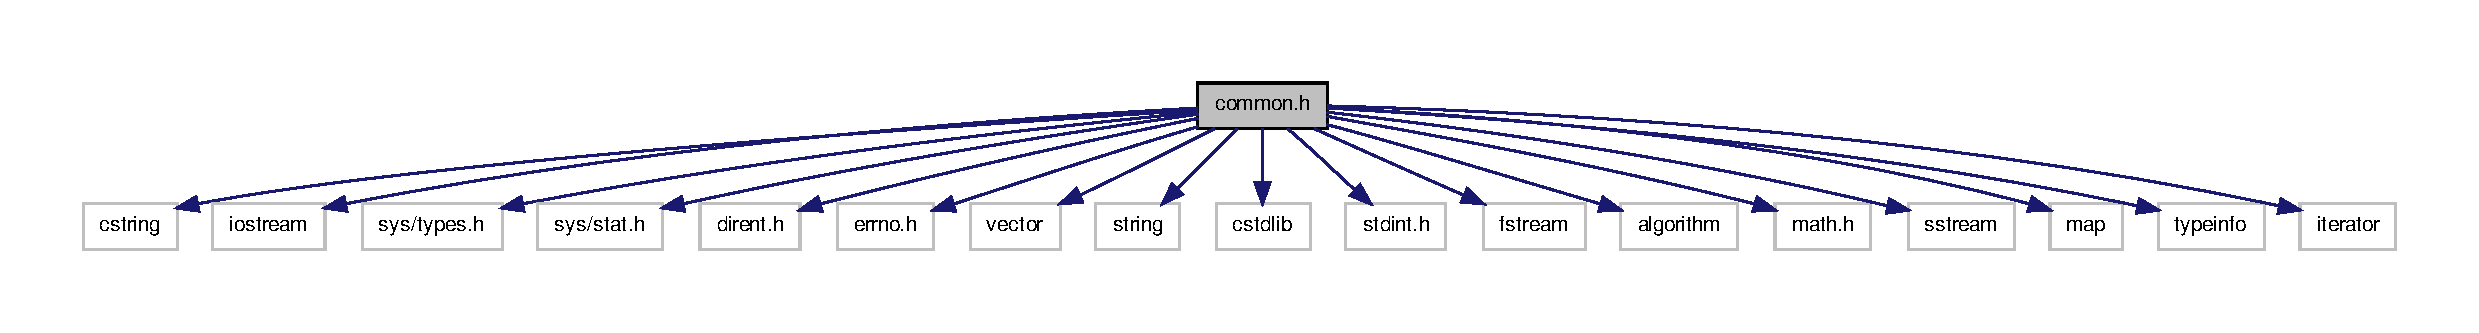
\includegraphics[width=400pt]{common_8h__incl}
\end{center}
\end{figure}
This graph shows which files directly or indirectly include this file:\nopagebreak
\begin{figure}[H]
\begin{center}
\leavevmode
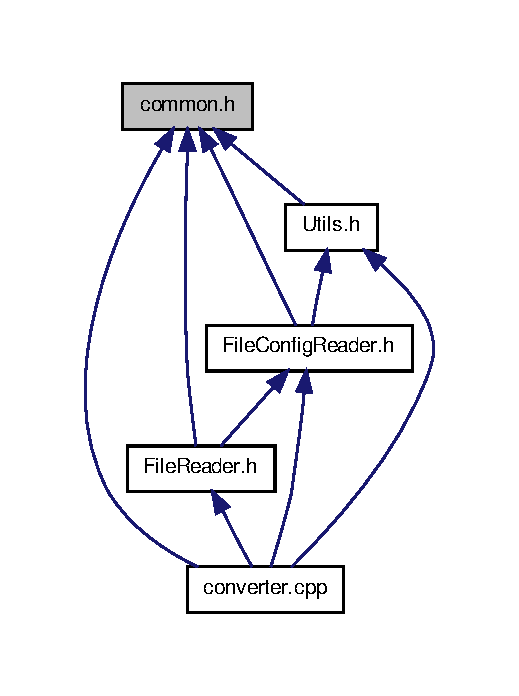
\includegraphics[width=249pt]{common_8h__dep__incl}
\end{center}
\end{figure}
\subsection*{Classes}
\begin{DoxyCompactItemize}
\item 
struct \hyperlink{structAgilentFileHeaderTag}{AgilentFileHeaderTag}
\begin{DoxyCompactList}\small\item\em The type used to represent the header of an Agilent file. \end{DoxyCompactList}\item 
struct \hyperlink{structAgilentWaveformHeaderTag}{AgilentWaveformHeaderTag}
\begin{DoxyCompactList}\small\item\em The type used to represent the header of each waveform in an Agilent file. \end{DoxyCompactList}\item 
struct \hyperlink{structAgilentWaveformDataHeaderTag}{AgilentWaveformDataHeaderTag}
\begin{DoxyCompactList}\small\item\em The type used to represent the data header of each waveform in an Agilent file. \end{DoxyCompactList}\end{DoxyCompactItemize}
\subsection*{Defines}
\begin{DoxyCompactItemize}
\item 
\hypertarget{common_8h_aefa6c5396054e382826a216d05be8226}{
\#define {\bfseries FILE\_\-TYPE\_\-LECROY}~1}
\label{common_8h_aefa6c5396054e382826a216d05be8226}

\item 
\hypertarget{common_8h_acd42695457b2e8440cb71a2aca3b40f5}{
\#define {\bfseries FILE\_\-TYPE\_\-AGILENT}~2}
\label{common_8h_acd42695457b2e8440cb71a2aca3b40f5}

\item 
\hypertarget{common_8h_a6bb41c0bfc0e8eadb604a630d027dcd4}{
\#define {\bfseries FILE\_\-TYPE\_\-TXT}~3}
\label{common_8h_a6bb41c0bfc0e8eadb604a630d027dcd4}

\item 
\hypertarget{common_8h_ae32b4bc47b1cc742b6f73d840bf8b2fa}{
\#define {\bfseries DATE\_\-TIME\_\-STRING\_\-LENGTH}~16}
\label{common_8h_ae32b4bc47b1cc742b6f73d840bf8b2fa}

\item 
\hypertarget{common_8h_aacee9a00efb3e5bc52594668c08fbf82}{
\#define {\bfseries FRAME\_\-STRING\_\-LENGTH}~24}
\label{common_8h_aacee9a00efb3e5bc52594668c08fbf82}

\item 
\hypertarget{common_8h_ad2f228ded688abd0adcc5013091e714a}{
\#define {\bfseries SIGNAL\_\-STRING\_\-LENGTH}~16}
\label{common_8h_ad2f228ded688abd0adcc5013091e714a}

\end{DoxyCompactItemize}
\subsection*{Typedefs}
\begin{DoxyCompactItemize}
\item 
typedef unsigned int \hyperlink{common_8h_a271e567655d46ec23cdcca42c1deab91}{UINTN}
\begin{DoxyCompactList}\small\item\em The type used to represent unsigned integer number. This value should be equal to 2$^\wedge$n. \end{DoxyCompactList}\item 
typedef struct \hyperlink{structAgilentFileHeaderTag}{AgilentFileHeaderTag} \hyperlink{common_8h_adbcbbec810f51100b2595f1395d60c3c}{AgilentFileHeader}
\begin{DoxyCompactList}\small\item\em The type used to represent the header of an Agilent file. \end{DoxyCompactList}\item 
typedef struct \hyperlink{structAgilentWaveformHeaderTag}{AgilentWaveformHeaderTag} \hyperlink{common_8h_a1f66db72c2c66ccb42604f224b7223e3}{AgilentWaveformHeader}
\begin{DoxyCompactList}\small\item\em The type used to represent the header of each waveform in an Agilent file. \end{DoxyCompactList}\item 
typedef struct \hyperlink{structAgilentWaveformDataHeaderTag}{AgilentWaveformDataHeaderTag} \hyperlink{common_8h_a5576fbb88d1a47675988d047621fdc92}{AgilentWaveformDataHeader}
\begin{DoxyCompactList}\small\item\em The type used to represent the data header of each waveform in an Agilent file. \end{DoxyCompactList}\end{DoxyCompactItemize}


\subsection{Detailed Description}
This file contains some commonly used includes, constants, defines, macros and typedefs. This file should be included by every .h file in the project.\par
 User should not change this file directly.\par
 The use of std namespace is declared.\par
 

\subsection{Typedef Documentation}
\hypertarget{common_8h_adbcbbec810f51100b2595f1395d60c3c}{
\index{common.h@{common.h}!AgilentFileHeader@{AgilentFileHeader}}
\index{AgilentFileHeader@{AgilentFileHeader}!common.h@{common.h}}
\subsubsection[{AgilentFileHeader}]{\setlength{\rightskip}{0pt plus 5cm}typedef struct {\bf AgilentFileHeaderTag} {\bf AgilentFileHeader}}}
\label{common_8h_adbcbbec810f51100b2595f1395d60c3c}


The type used to represent the header of an Agilent file. 

The struct represents the equivalent header of an Agilent file \hypertarget{common_8h_a5576fbb88d1a47675988d047621fdc92}{
\index{common.h@{common.h}!AgilentWaveformDataHeader@{AgilentWaveformDataHeader}}
\index{AgilentWaveformDataHeader@{AgilentWaveformDataHeader}!common.h@{common.h}}
\subsubsection[{AgilentWaveformDataHeader}]{\setlength{\rightskip}{0pt plus 5cm}typedef struct {\bf AgilentWaveformDataHeaderTag} {\bf AgilentWaveformDataHeader}}}
\label{common_8h_a5576fbb88d1a47675988d047621fdc92}


The type used to represent the data header of each waveform in an Agilent file. 

The struct represents the equivalent data header of a waveform in an Agilent file \hypertarget{common_8h_a1f66db72c2c66ccb42604f224b7223e3}{
\index{common.h@{common.h}!AgilentWaveformHeader@{AgilentWaveformHeader}}
\index{AgilentWaveformHeader@{AgilentWaveformHeader}!common.h@{common.h}}
\subsubsection[{AgilentWaveformHeader}]{\setlength{\rightskip}{0pt plus 5cm}typedef struct {\bf AgilentWaveformHeaderTag} {\bf AgilentWaveformHeader}}}
\label{common_8h_a1f66db72c2c66ccb42604f224b7223e3}


The type used to represent the header of each waveform in an Agilent file. 

The struct represents the equivalent header of a waveform in an Agilent file \hypertarget{common_8h_a271e567655d46ec23cdcca42c1deab91}{
\index{common.h@{common.h}!UINTN@{UINTN}}
\index{UINTN@{UINTN}!common.h@{common.h}}
\subsubsection[{UINTN}]{\setlength{\rightskip}{0pt plus 5cm}typedef unsigned int {\bf UINTN}}}
\label{common_8h_a271e567655d46ec23cdcca42c1deab91}


The type used to represent unsigned integer number. This value should be equal to 2$^\wedge$n. 


\hypertarget{converter_8cpp}{
\section{converter.cpp File Reference}
\label{converter_8cpp}\index{converter.cpp@{converter.cpp}}
}


This is the file containing the main of the program.  


{\ttfamily \#include \char`\"{}common.h\char`\"{}}\par
{\ttfamily \#include \char`\"{}FileReader.h\char`\"{}}\par
{\ttfamily \#include \char`\"{}FileConfigReader.h\char`\"{}}\par
{\ttfamily \#include \char`\"{}Utils.h\char`\"{}}\par
Include dependency graph for converter.cpp:\nopagebreak
\begin{figure}[H]
\begin{center}
\leavevmode
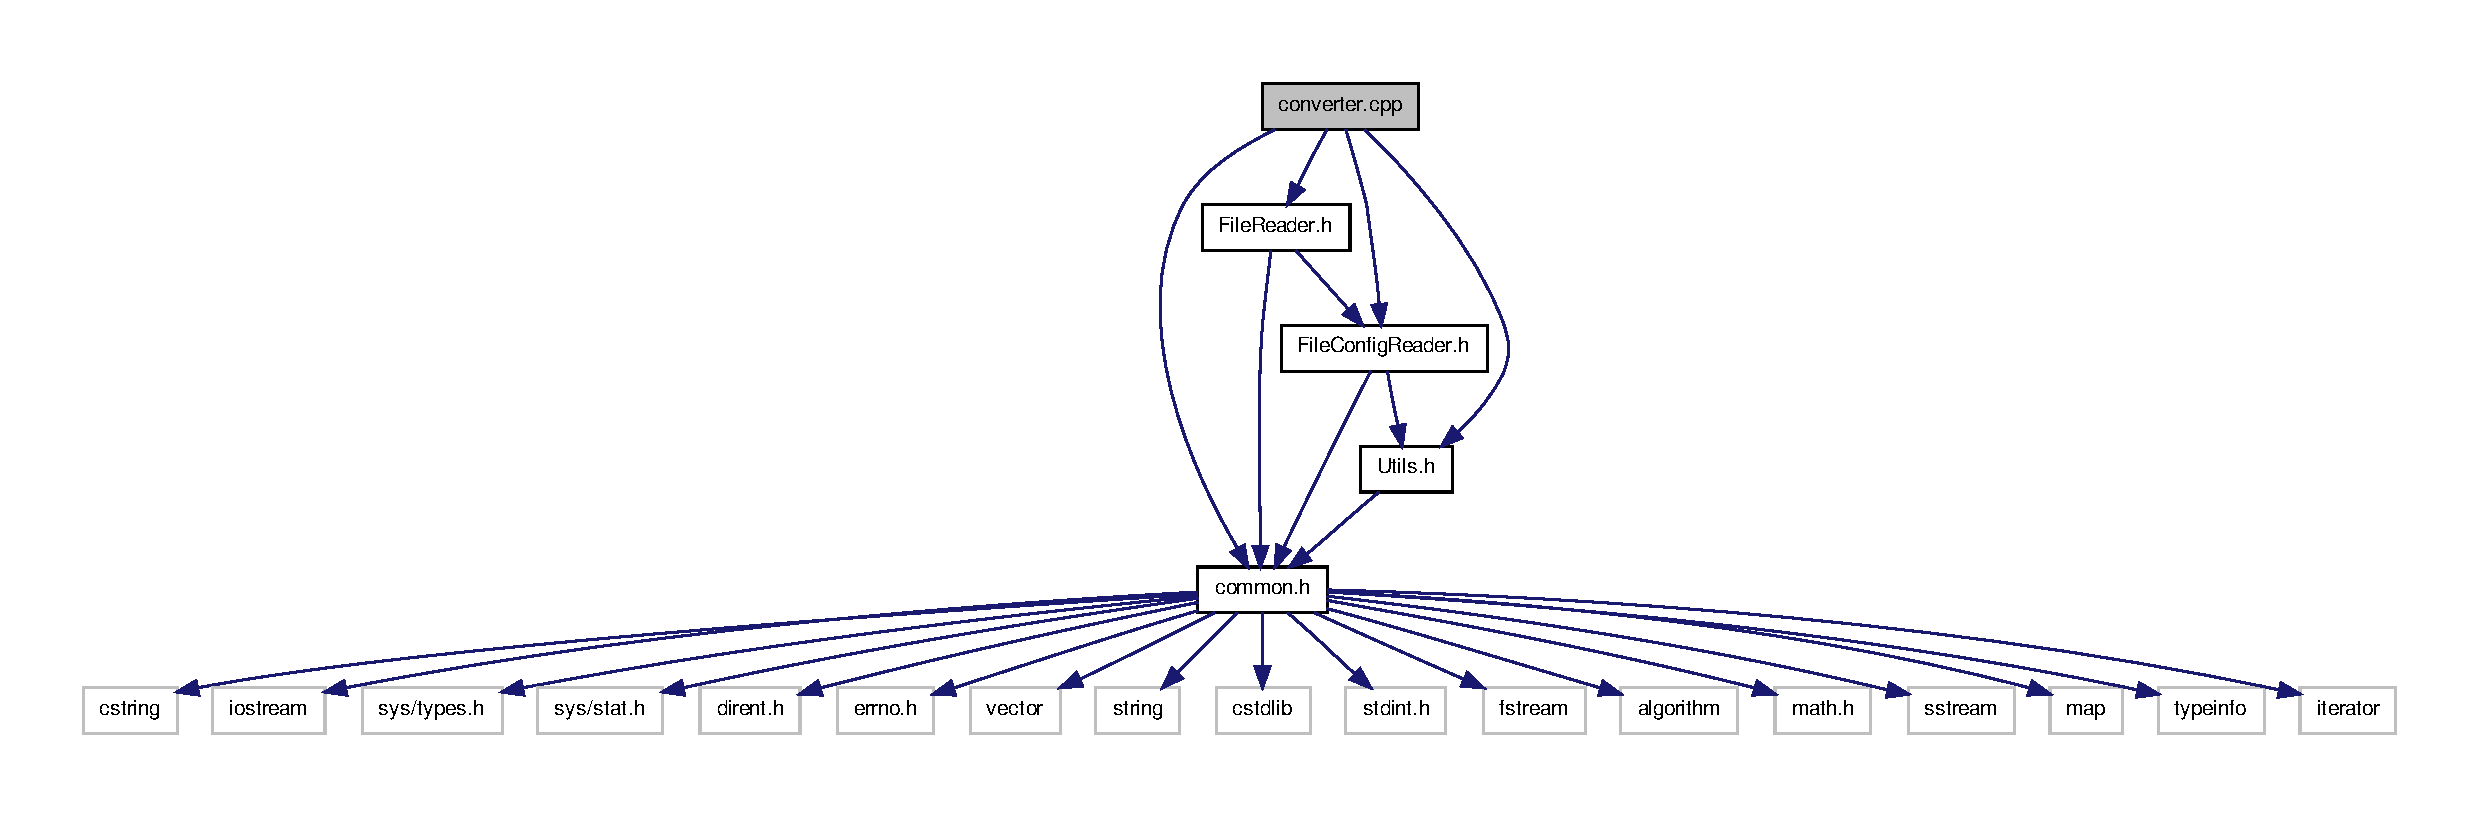
\includegraphics[width=400pt]{converter_8cpp__incl}
\end{center}
\end{figure}
\subsection*{Functions}
\begin{DoxyCompactItemize}
\item 
void \hyperlink{converter_8cpp_a97ee70a8770dc30d06c744b24eb2fcfc}{help} ()
\begin{DoxyCompactList}\small\item\em Prints help informations. \end{DoxyCompactList}\item 
int \hyperlink{converter_8cpp_a0ddf1224851353fc92bfbff6f499fa97}{main} (int argc, char $\ast$argv\mbox{[}$\,$\mbox{]})
\begin{DoxyCompactList}\small\item\em Main function of the program. \end{DoxyCompactList}\end{DoxyCompactItemize}


\subsection{Detailed Description}
This is the file containing the main of the program. 

\subsection{Function Documentation}
\hypertarget{converter_8cpp_a97ee70a8770dc30d06c744b24eb2fcfc}{
\index{converter.cpp@{converter.cpp}!help@{help}}
\index{help@{help}!converter.cpp@{converter.cpp}}
\subsubsection[{help}]{\setlength{\rightskip}{0pt plus 5cm}void help (
\begin{DoxyParamCaption}
{}
\end{DoxyParamCaption}
)}}
\label{converter_8cpp_a97ee70a8770dc30d06c744b24eb2fcfc}


Prints help informations. 

\hypertarget{converter_8cpp_a0ddf1224851353fc92bfbff6f499fa97}{
\index{converter.cpp@{converter.cpp}!main@{main}}
\index{main@{main}!converter.cpp@{converter.cpp}}
\subsubsection[{main}]{\setlength{\rightskip}{0pt plus 5cm}int main (
\begin{DoxyParamCaption}
\item[{int}]{argc, }
\item[{char $\ast$}]{argv\mbox{[}$\,$\mbox{]}}
\end{DoxyParamCaption}
)}}
\label{converter_8cpp_a0ddf1224851353fc92bfbff6f499fa97}


Main function of the program. 


\begin{DoxyParams}{Parameters}
{\em argc} & \\
\hline
{\em argv} & \\
\hline
\end{DoxyParams}
\begin{DoxyReturn}{Returns}
0 if everything went fine 
\end{DoxyReturn}

\hypertarget{FileConfigReader_8h}{
\section{FileConfigReader.h File Reference}
\label{FileConfigReader_8h}\index{FileConfigReader.h@{FileConfigReader.h}}
}
{\ttfamily \#include \char`\"{}common.h\char`\"{}}\par
{\ttfamily \#include \char`\"{}Utils.h\char`\"{}}\par
Include dependency graph for FileConfigReader.h:\nopagebreak
\begin{figure}[H]
\begin{center}
\leavevmode
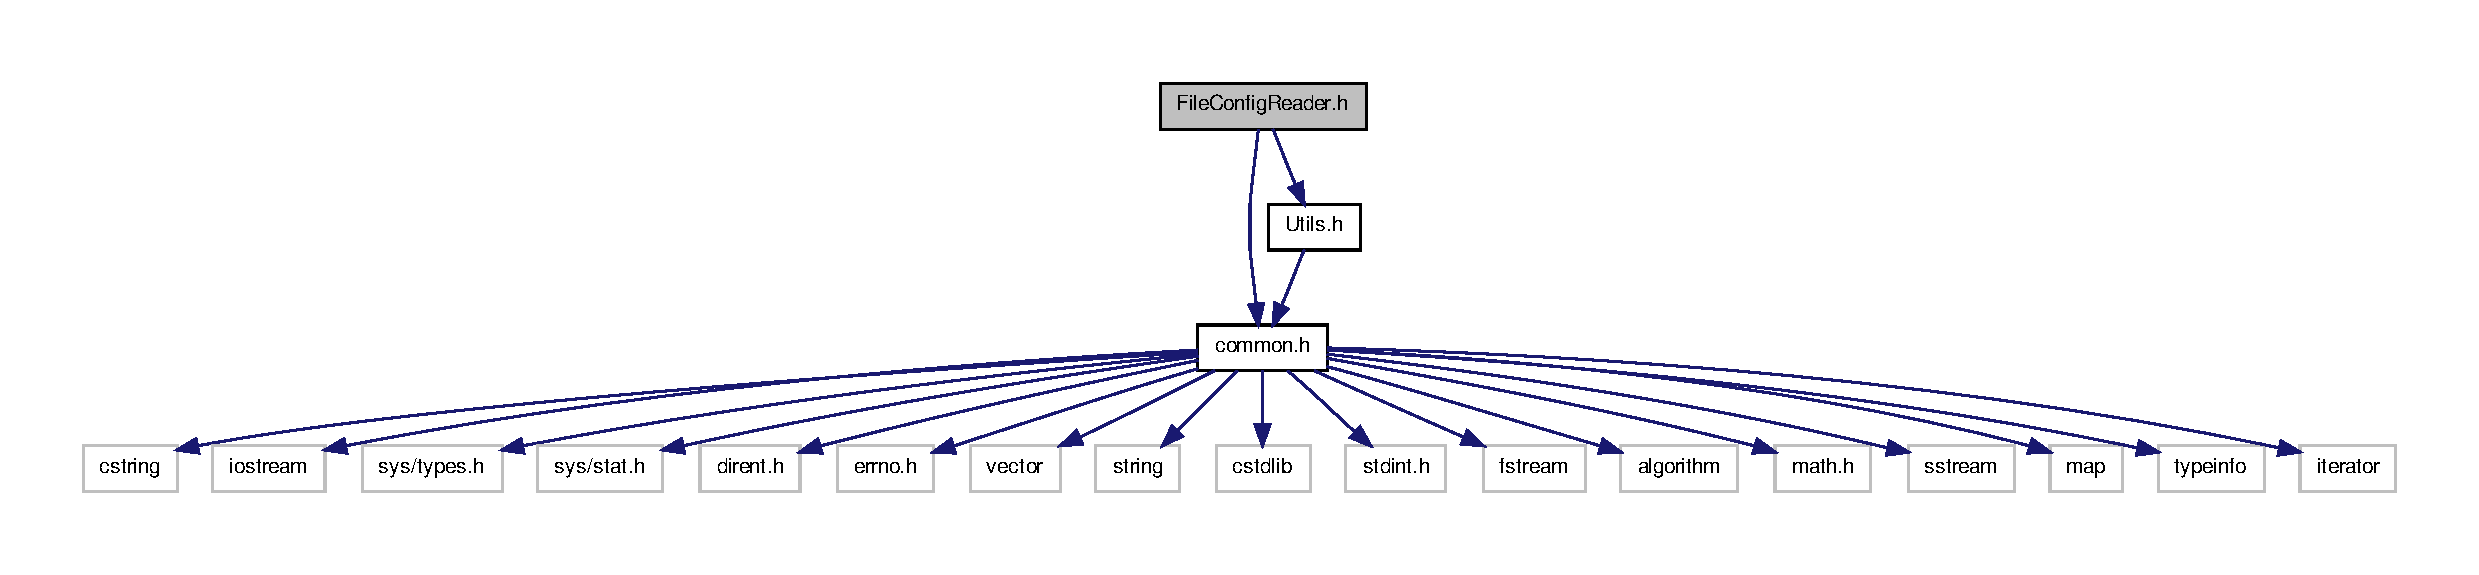
\includegraphics[width=400pt]{FileConfigReader_8h__incl}
\end{center}
\end{figure}
This graph shows which files directly or indirectly include this file:\nopagebreak
\begin{figure}[H]
\begin{center}
\leavevmode
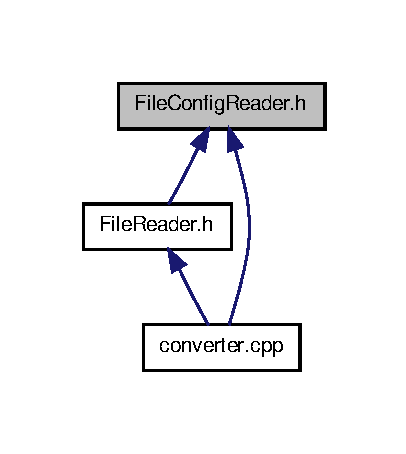
\includegraphics[width=195pt]{FileConfigReader_8h__dep__incl}
\end{center}
\end{figure}
\subsection*{Classes}
\begin{DoxyCompactItemize}
\item 
class \hyperlink{classFileConfigReader}{FileConfigReader}
\begin{DoxyCompactList}\small\item\em This class parses a converter configuration file. \end{DoxyCompactList}\end{DoxyCompactItemize}


\subsection{Detailed Description}

\hypertarget{FileReader_8h}{
\section{FileReader.h File Reference}
\label{FileReader_8h}\index{FileReader.h@{FileReader.h}}
}
{\ttfamily \#include \char`\"{}common.h\char`\"{}}\par
{\ttfamily \#include \char`\"{}FileConfigReader.h\char`\"{}}\par
Include dependency graph for FileReader.h:\nopagebreak
\begin{figure}[H]
\begin{center}
\leavevmode
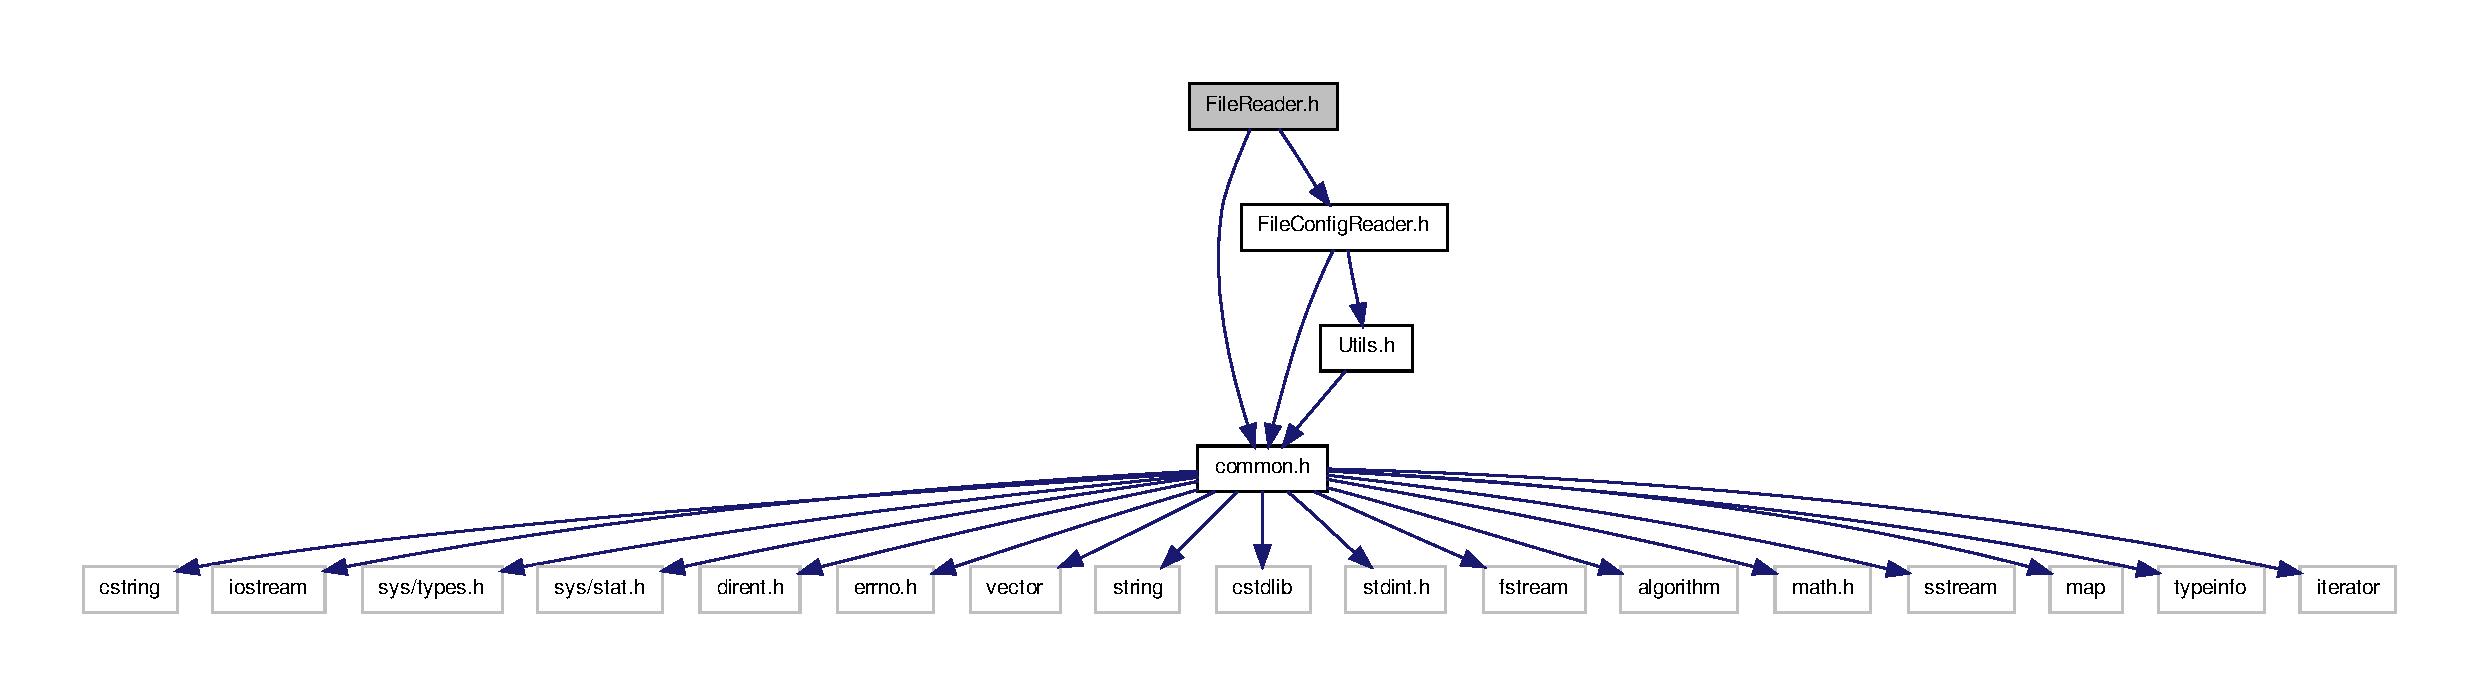
\includegraphics[width=400pt]{FileReader_8h__incl}
\end{center}
\end{figure}
This graph shows which files directly or indirectly include this file:\nopagebreak
\begin{figure}[H]
\begin{center}
\leavevmode
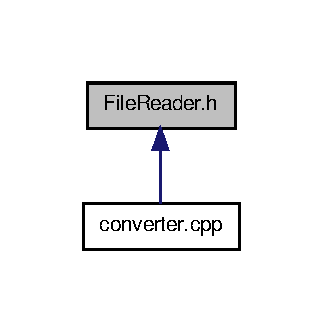
\includegraphics[width=154pt]{FileReader_8h__dep__incl}
\end{center}
\end{figure}
\subsection*{Classes}
\begin{DoxyCompactItemize}
\item 
class \hyperlink{classFileReader}{FileReader}
\begin{DoxyCompactList}\small\item\em This class parses Lecroy or Agilent files. \end{DoxyCompactList}\end{DoxyCompactItemize}


\subsection{Detailed Description}

\hypertarget{Utils_8h}{
\section{Utils.h File Reference}
\label{Utils_8h}\index{Utils.h@{Utils.h}}
}
{\ttfamily \#include \char`\"{}common.h\char`\"{}}\par
Include dependency graph for Utils.h:\nopagebreak
\begin{figure}[H]
\begin{center}
\leavevmode
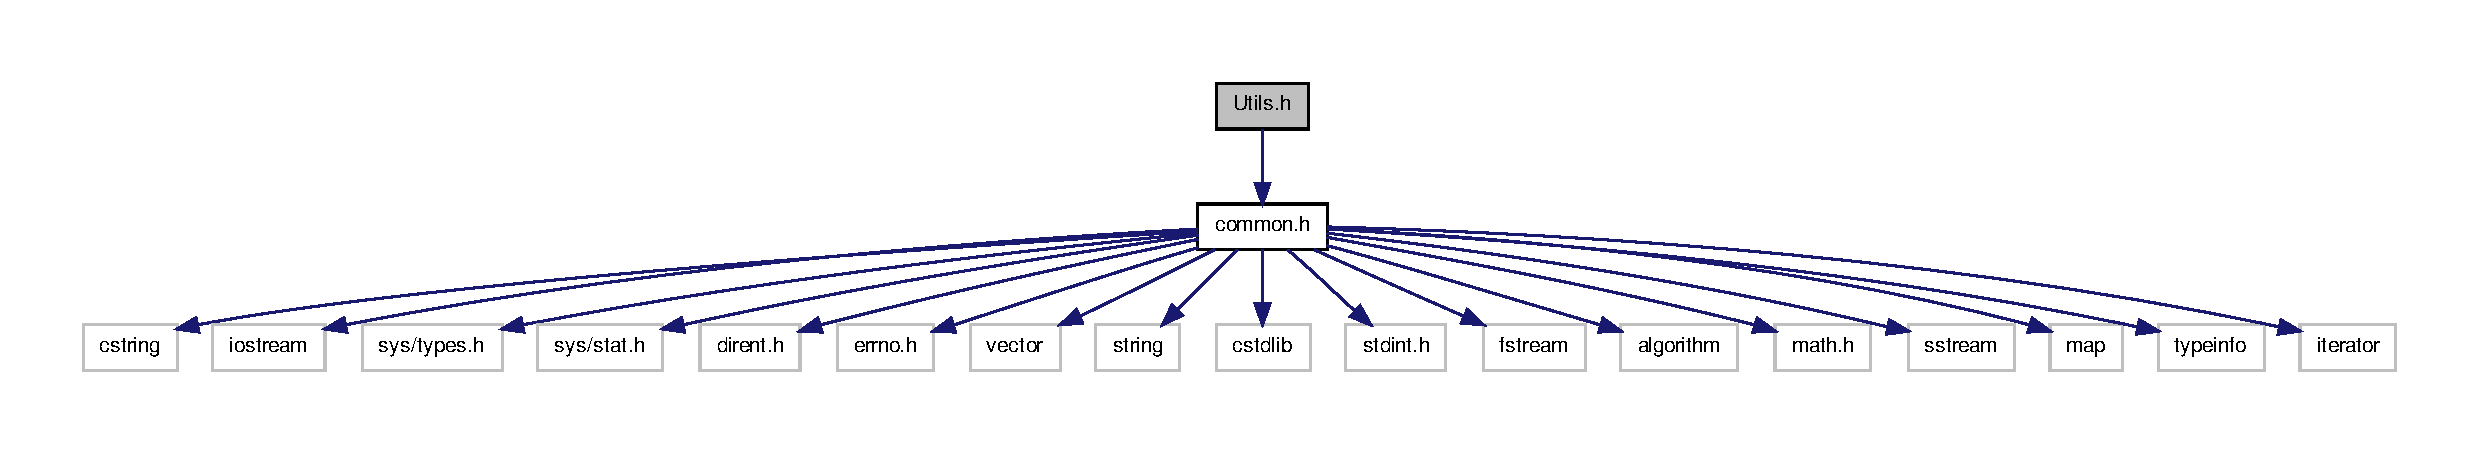
\includegraphics[width=400pt]{Utils_8h__incl}
\end{center}
\end{figure}
This graph shows which files directly or indirectly include this file:\nopagebreak
\begin{figure}[H]
\begin{center}
\leavevmode
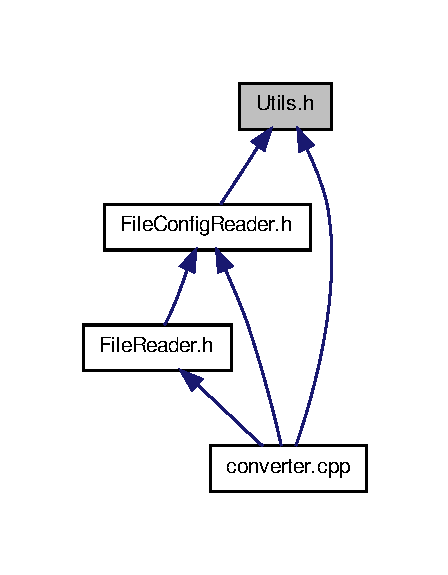
\includegraphics[width=215pt]{Utils_8h__dep__incl}
\end{center}
\end{figure}
\subsection*{Classes}
\begin{DoxyCompactItemize}
\item 
class \hyperlink{classUtils}{Utils}
\begin{DoxyCompactList}\small\item\em This class provides some helpful static functions. \end{DoxyCompactList}\end{DoxyCompactItemize}


\subsection{Detailed Description}

\printindex
\end{document}
